\documentclass[conference]{IEEEtran}
\IEEEoverridecommandlockouts
% The preceding line is only needed to identify funding in the first footnote. If that is unneeded, please comment it out.
\usepackage{cite}
\usepackage{amsmath,amssymb,amsfonts}
\usepackage{algorithmic}
\usepackage{graphicx}
\usepackage{textcomp}
\usepackage{xcolor}
\usepackage{multirow}
\usepackage[numbers,sort&compress]{natbib}
%\usepackage{natbib}
%\usepackage{ulem}
\def\BibTeX{{\rm B\kern-.05em{\sc i\kern-.025em b}\kern-.08em
    T\kern-.1667em\lower.7ex\hbox{E}\kern-.125emX}}
\begin{document}

\title{Confidence map based KCF object tracking algorithm\\
%{\footnotesize \textsuperscript{*}Note: Sub-titles are not captured in Xplore and
%should not be used}
\thanks{Science and Technology Research Program of Xi'an (2017086CG/RC049), China.}
\thanks{Key Science and Technology Program of Guizhou Province (2017GZ60903), China}
}

\author{\IEEEauthorblockN{1\textsuperscript{st} Baoguo Wei}
\IEEEauthorblockA{\textit{School of Electronic Information} \\
\textit{Northwestern Polytechnical University}\\
Xi'an, China \\
Wbg@nwpu.edu.cn}
\and
\IEEEauthorblockN{2\textsuperscript{nd} Yufei Wang}
\IEEEauthorblockA{\textit{School of Electronic Information} \\
\textit{Northwestern Polytechnical University}\\
Xi'an, China \\
18435169138@mail.nwpu.edu.cn}
\and
\IEEEauthorblockN{3\textsuperscript{rd} Xingjian He}
\IEEEauthorblockA{\textit{School of Electronic Information} \\
\textit{Northwestern Polytechnical University}\\
Xi'an, China \\
2014302129@mail.nwpu.edu.cn}
}

\maketitle

\begin{abstract}
Tracking with kernelized correlation filters (KCF) is an excellent object tracking algorithm, which is widely concerned.
However, it still has many limitations, such as its tracking performance decreases in complex scenes, and the model is easily contaminated because it is updated every frame.
In KCF, each candidate patch in tracked region corresponds to a confidence ratio reflecting the probability that it contains the target, and the tracking patch corresponding with the maximum confidence ratio is the output.
We combine all available confidence ratios to obtain a confidence map and infer the tracking scene by analyzing the confidence map.
For complex scenes, we dynamically improve KCF to enhance its tracking performance.
In addition, we propose an innovative model update mechanism to reduce the computational complexity and model contamination. 
The experimental results show that compared with the conventional KCF algorithm, the proposed approach improves success rate and precision by 7\% and 8\% respectively.
\end{abstract}

\begin{IEEEkeywords}
object tracking, confidence map, kernelized correlation filter, model update mechanism
\end{IEEEkeywords}

\section{INTRODUCTION}
Object tracking is a classic problem in computer vision, which has a wide range of applications. \cite{Survey,Survey2}. 
However, it is still difficult due to many challenging aspects, such as occlusion, fast motion, similar target and deformation.

In recent years, many object tracking algorithms based on discriminative learning method are proposed and have made a lot of process \cite{Discriminative}. 
In 2015, Henriques proposed KCF (Tracking with Kernelized Correlation Filters) algorithm \cite{KCF}. 
It obtains periodic training samples by cyclically shifting the image and simplifies the calculation process using DFT (Discrete Fourier Transform). 
"Kernel trick" is simultaneously employed to improve its tracking performance. 
However, KCF uses the same tracking mechanism in different scenes, it can track accurately in simple scenes, but its tracking performance decreases in complex scenes.
When faced tracking scenes with similar target, background clutter or motion blur, it is difficult for KCF to use a single HOG (Histogram of Oriented Gradients) feature to effectively describe the target.
When faced tracking scenes with occlusion or fast motion, the limited tracked region in KCF also impairs tracking performance.
In addition, KCF model is updated every frame, it is computationally intensive and easily causes model contaminant.

Based on these observations, we propose an improved KCF algorithm based on confidence map.
The novelty of our work is that:
\begin{itemize}
\item A confidence map is proposed. The confidence map reflects all available confidence ratios. According to the peak response types of the confidence map, we can deduce the type of the tracking scene and the challenging aspects that may be included.  
\item An improved KCF algorithm is proposed for complex tracking scenes.
When faced tracking scenes with similar target, background clutter or motion blur, we combine the color features and HOG features to effectively describe the target.
When faced tracking scenes with occlusion or fast motion, we expand the tracked region to improve the tracking performance.
\item A model update mechanism is proposed based on the extent of target deformation.
The proposed deformation index determines whether the model needs to be updated.
The algorithm model is no longer updated every frame, which reduces the amount of calculation and model contamination. 
\end{itemize}
The experimental results show that compared with the conventional KCF algorithm, the proposed approach improves success rate and precision by 7\% and 8\% respectively.

The rest of this paper is organized in five sections. The second part describes the related works. The third part presents the enhanced algorithm. The fourth part reports the results of the experiment. Finally, the fifth part makes a summary and introduces the future work.
\begin{figure*}[htbp]
	\centering
	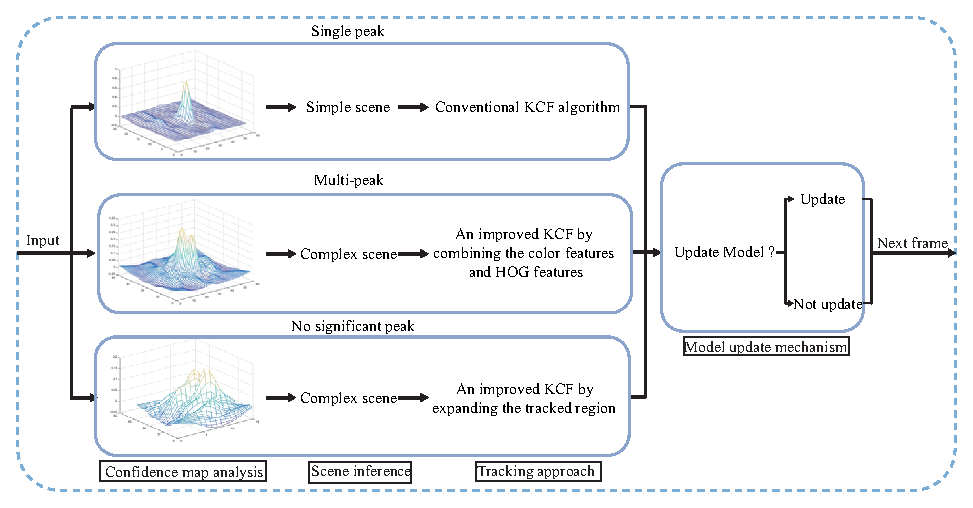
\includegraphics[scale=1]{flow.eps}
	\caption{The flow chart of confidence map based KCF algorithm}
	\label{fig:flow}
\end{figure*}

\section{RELATED WORKS}
In this section, we will discuss discriminative object tracking algorithms and confidence ratio.

One of the biggest breakthroughs in recent object tracking research was the adoption of discriminative learning methods. 
Discriminative object tracking algorithms regard tracking as an online learning problem.
It employs the target area as positive samples and the background area as negative samples to learn a classifier.
The classifier can discriminate between the target and surrounding environment to achieve object tracking.
Typical examples of classifiers include SVM (Support Vector Machines) \cite{SVM}, random forest classifiers \cite{Randomforest} and boosting variants \cite{Boosting}.

The classifier after learning is tested on many candidate patches of the tracked region to find the most likely target location \cite{confidencemap}. 
For a specific classifier, every candidate patch will obtain a classification probability reflecting the possibility that it contains the target. 
In this paper, we use the confidence ratio to represent the classification probability.
KCF generally considers the patch corresponding to the maximum confidence ratio as target location.
We combine all available confidence ratios to obtain a confidence map, it expresses the probability that any candidate patch in the tracked region contains the target.



\section{THE PROPOSED APPROACH}
The proposed approach is shown in Fig.~\ref{fig:flow}.
We first obtain the confidence map of the input image.
By analyzing the local maximum of the confidence map, we class it into three peak response types: single peak confidence map, multi-peak confidence map and the confidence map with no significant peak.
For each type, we infer the complexity of the tracking scene and the challenging aspects that may be included.
Then, different tracking approaches are employed to improve the tracking performance of KCF.
Finally, we use the proposed model update mechanism to determine whether the model needs to be updated.
In this section, we introduce the proposed approach from three parts: KCF algorithm, tracking based on confidence map and model update mechanism. 

\subsection{KCF algorithm}
The core component of KCF is a discriminative classifier $f(z)={\rm w}^{T}z$ which discriminates between the target and surrounding environment.
For object tracking, the target location is given in the first frame of the video sequence.
KCF extracts the HOG feature \cite{HOG} of the target and obtains training samples by cyclic shift.
${\rm x}=[x_1,x_2,\cdots,x_n]^T$ is a HOG feature array, circulating shift it as $P_{\rm x}^1=[x_n,x_1,x_2,\cdots,x_{n-1}]^T$.
All loop shifted samples $\{P_{\rm x}^u|u=0,\cdots,n-1\}$ constitute a circulant matrix ${\rm X}=C({\rm x})$. 
KCF uses the fact that the circulant matrix can be diagonalized by DFT.
\begin{equation}
X=F^{H}{\rm diag}(\hat{{\rm x}})F
\label{KCF1}
\end{equation} 
Where $F$ represents the DFT matrix which computes the DFT of any input vector, as $\mathcal{F}({\rm x})=\sqrt{n}F{\rm x}$, $F^H$ is the Hermitian transpose matrix of $F$. From now on, a hat $\hat{}$ is used as shorthand for the DFT of a vector. 

For Ridge Regression, we can obtain ${\rm w}=({\rm X}^{T}{\rm X} +\lambda I)^{-1}X^{T}y$ by \eqref{KCF2}, where ${\rm x}_i$ is a sample and $y_i$ is its regression target.
\begin{equation}
\mathop{\min}_{{\rm w}}\sum_{i}^{}(f({\rm x}_i)-y_i)^2+\lambda\|{\rm w}\|
\label{KCF2}
\end{equation}
We define the element-wise product as $\bigodot$.
Since $X$ is a circulant matrix, ${\rm w}$ shown in \eqref{KCF3} can be obtained.
\begin{equation}
\hat{{\rm w}}=\frac{\hat{{\rm x}}^*\bigodot \hat{y}}{\hat{{\rm x}}^*\bigodot \hat{{\rm x}}+\lambda}
\label{KCF3}
\end{equation}

"Kernel trick" is employed for non-linear regression.
The solution of the kernel function can be transformed into a linear combination of samples: ${\rm w}=\sum_{i} \alpha_i \varphi(x_i)$, translates into solving $\alpha=\{\alpha_1,\alpha_2,\cdots,\alpha_n\}^T$. After the diagonalization of the kernel matrix, the Gauss kernel function can be used to obtain as follow:
\begin{equation}
	\hat{\alpha}=\frac{\hat{y}}{\hat{k}^{{\rm xx}}+\lambda}
	\label{KCF4}
\end{equation}
For any two vectors ${\rm x}$ and ${\rm x}'$, their kernel function related operations from the $k^{{\rm xx}'}$, the $i$ element of vector $k^{{\rm xx}'}$ is $k^{{\rm xx}'}=k({\rm x}',P^{i-1}{\rm x})$, $k^{{\rm xx}'}$ is two parameters of different relative displacements evaluated in the kernel. The use of Gauss kernels for $k^{{\rm xx}'}$ yields the following expression:
\begin{equation}
	\hat{k}^{{\rm xx'}}={\rm exp}(-\frac{1}{\sigma^2}(\|{\rm x}\|^2+\|{\rm x}'\|^2)-2F^{-1}(\hat{{\rm x}}\bigodot\hat{{\rm x}}^{'*}))
	\label{KCF5}
\end{equation}

For the KCF algorithm using the Gauss kernel function, the HOG feature of the image is extracted first, and the $\sigma$ in the kernel function of the algorithm is calculated, and the $\lambda$ in the $\alpha$ is calculated to train the samples. The intensive sampling of the tracked region is used to calculate the correlation between the samples to be measured, and the target location of the frame is obtained. 

\subsection{Tracking based on confidence map}
The confidence map is classed into three different peak response types: single peak confidence map, multi-peak confidence map and the confidence map with no significant peak.
We check in order which type the confidence map belongs to and infer its corresponding scene.
For different scenes, we employ different tracking approaches.

\subsubsection{Single peak confidence map}
if the confidence map has a local maximum $m_i$ which satisfies \eqref{Model1}, it is considered as a single peak confidence map.
\begin{equation}
	\frac{m_i}{m_j}\geqslant \varepsilon, \forall i\neq j
	\label{Model1}
\end{equation}
Where $m_j$ is any local maximum of the confidence map other than $m_i$, $\varepsilon$ is the threshold of the peak ratio we set it to $1.5$.
The single peak confidence map and its corresponding tracking scene are shown in Fig.~\ref{fig:1}.
\begin{figure}[htbp]
	\centering
	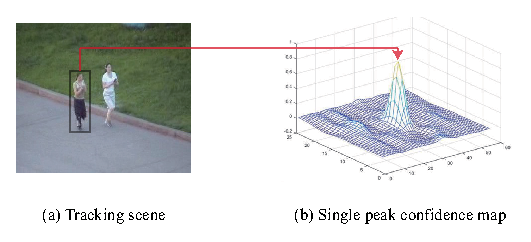
\includegraphics[scale=1]{con1.eps}
	\caption{Single peak confidence map and its corresponding tracking scene}
	\label{fig:1}
\end{figure}

\noindent
{\bfseries Confidence map analysis:} only one candidate patch can be identified as the tracking target, and the probability is high.

\noindent
{\bfseries Scene inference:} simple scene.

\noindent
{\bfseries Tracking approach:} KCF algorithm. The patch corresponding to the maximum of the confidence map is output as the target.

\subsubsection{Multi-peak confidence map}
if the confidence map has multiple local maxima (more than one) greater than the threshold of the peak, we set it to $0.6$, and any two of these local maxima satisfy \eqref{Model2}, it is considered as multi-peak confidence map.
\begin{equation}
   \frac{m_i}{m_j}< \varepsilon, \forall i\neq j
   \label{Model2}
\end{equation}
Where $\varepsilon$ is the same threshold as the previous section. The multi-peak confidence map and its corresponding tracking scene are shown in Fig.~\ref{fig:2}.
\begin{figure}[htbp]
	\centering
	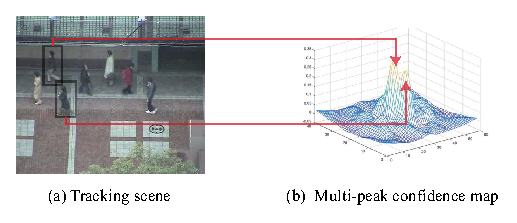
\includegraphics[width=9cm]{con2.eps}
	\caption{Multi-peak confidence map and its corresponding tracking scene}
	\label{fig:2}
\end{figure}

\noindent
{\bfseries Confidence map analysis:} multiple candidate patches can be identified as the tracking target, and their probabilities are similar.

\noindent
{\bfseries Scene inference:} complex scenes with similar targets, background clutter or motion blur.

\noindent
{\bfseries Tracking approach:} an improve KCF algorithm by combining the color features and HOG features.
The color information is widely used in object tracking because it describes the target well \cite{colorinformation}.
More importantly, it is independent and complementary to the HOG feature adopted by KCF \cite{color2}.
Therefore, we add the color histogram feature to the original model of KCF to build a more robust object model.
It compensates for the inability of KCF to accurately track in the above tracking scenes.

If the t-th frame is a color image, we convert it from the RGB color space to the Lab color space.
The information of three channels (L channel, a channel and b channel) is extracted and combined into a color histogram.
If the image is a grayscale image, the information of L channel is extracted to form a color histogram.
Because the time interval between two adjacent frames is small, their color information is similar.
We calculate the color histogram similarity between the candidate patches of the t-th frame and the estimated target of the (t-1)th frame by \eqref{Model3}.
\begin{equation}
	\rho = \frac{1}{d({\rm c}_{t-1}^{target},{\rm c}_t^{i})}
	\label{Model3}
\end{equation}
Where ${\rm c}_{t-1}^{target}$ is the color histogram feature of the estimated target of the (t-1)th frame, ${\rm c}_t^{i}$ is the color histogram feature of candidate patches in the t-th frame, $d({\rm c}_{t-1}^{target},{\rm c}_t^i)$ is the Euclidean distance between them.
$\rho$ is normalized to obtain the confidence ratio of the candidate patches under the color histogram feature, denoted as $g(z)$.
We combine it and the confidence ratio under the HOG feature $f(z)$ and to obtain the final confidence ratio $s(z)$ by \eqref{Model4}.
\begin{equation}
	s(z)=0.5f(z)+0.5g(z)
	\label{Model4}
\end{equation}
The patch corresponding to the maximum of $s(z)$ is output as the target.

\begin{figure*}[t]
	\centering
	\includegraphics[scale=1]{quality.eps}
	\caption{The tracking results of different algorithms on the same video sequence (from top to bottom are Woman, Coke, Couple and Surfer).}
	\label{fig:qual}
\end{figure*}


\subsubsection{The confidence map with no significant peak}
if the confidence map is neither single peak nor multi-peak, we consider it as the confidence map with no significant peak.
The confidence map with no significant peak and its corresponding tracking scene are shown in Fig.~\ref{fig:3}.
\begin{figure}[htbp]
	\centering
	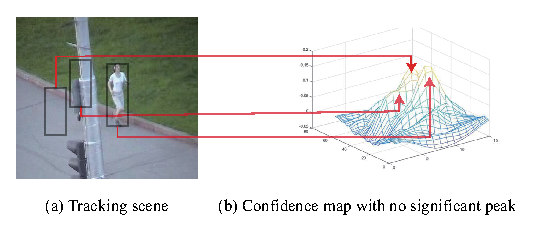
\includegraphics[scale=1]{con3.eps}
	\caption{The confidence map with no significant peak and its corresponding tracking scene}
	\label{fig:3}
\end{figure}

\noindent
{\bfseries Confidence map analysis:} no candidate image patch can be identified as the tracking target.

\noindent
{\bfseries Scene inference:} complex scenes with occlusion or fast motion.

\noindent
{\bfseries Tracking approach:} an improve KCF by expanding the tracked region.
Double the tracked region of the conventional KCF.
The improved algorithm is more likely to track successfully in the above scenes.


\subsection{Model update mechanism}
During the tracking process, the target will be deformed, the algorithm model needs to be constantly updated \cite{Modelupdate}.
The KCF model is updated every frame.
In this way, the calculation is very heavy and the model is easily contaminated.
We propose an innovative model update mechanism to address the problem, whether the model is updated depends on the extent of target deformation.

The first frame of the video sequence contains the complete information of the target.
The extent of target deformation can be measured by calculating the difference between the estimated target of the current frame and the given target of the first frame.
Since KCF extracts the HOG feature of each frame, the deformation extent $d$ can be obtained by \eqref{Update1}.
\begin{equation}
	d=d({\rm x}_1,{\rm x}_t)
	\label{Update1}
\end{equation}
Where ${\rm x}_1$ is the HOG feature of the given target of the first frame, ${\rm x}_t$ is the HOG feature of the estimated target of the current frame, $d({\rm x}_1,{\rm x}_t)$ is the Euclidean distance between them. 
If $d$ is greater than the threshold we set it to 1.5, it means the deformation of the target is large enough to update the model.
The model update method is the same as KCF method.

\section{EXPERIMENTS}

We implement our method with MATLAB on a desktop computer with Inter Core i5, 3.20GHz, 4GB RAM. 
The video sequences we use come from OTB (Visual tracker benchmark) dataset \cite{OTB}.
The proposed approach denoted by CMKCF is compared with related state-of-the-art algorithms such as KCF \cite{KCF}, TLD \cite{TLD}, CT \cite{CT}, CSK \cite{CSK}.
Experimental results show that CMKCF has a better tracking performance.

\subsection{Quality evaluation}
To evaluate the proposed approach, we compare the experimental result of CMKCF with the results of KCF \cite{KCF}, TLD \cite{TLD}, CT \cite{CT}, CSK \cite{CSK}.
Fig.~\ref{fig:qual} shows the tracking results of different algorithms on the same video sequence.
The video sequences we use are  Woman, Coke, Couple and Surfer.

For Woman, we track a woman who is walking along the road, it means that the target is constantly deformed.
At approximately 136th frame, the target is occluded by a white car, TLD and CT fail to track.
At approximately 571th frame, KCF also fails to track, CMKCF still accurately tracks the target.
The experimental results show that CMKCF has a better performance compared to other algorithms in this video sequence.

In Coke, a canister in the hand of a man is determined as the tracking target.
In this video sequence, occlusion and fast motion occur simultaneously.
At approximately 250th frame, CT is slightly offset, TLD and CSK start to drift.
At approximately 271th frame, the tracking boxes of TLD, KCF, CT and CSK all drift, only CMKCF accurately tracks the target.

For Couple, the tracking scene with similar targets and background clutter is complex.
At approximately 25th frame, only CMKCF and KCF accurately track the target.
At approximately 40th frame, KCF using a single HOG feature does not describe the target well, its tracking box seriously deviates from the target.
From this frame, only CMKCF can accurately track the target.
It means that CMKCF has a stable performance on this video sequence.

In surfer, the main challenging aspect is fast motion.
Faced with this challenging aspect, CT and CSK, at approximately 108th frame, fail to track the target.
At approximately 138th frame, the target is not in the tracked region of KCF due to fast motion, the tracking box of KCF starts to drift.
However, CMKCF expanding the tracked region of KCF accurately tracks the target.

\begin{figure}[t]
	\centering
	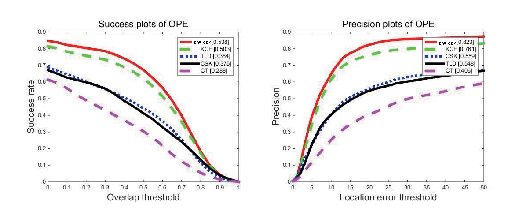
\includegraphics[width=9cm]{quantity.eps}
	\caption{The experimental results of the proposed algorithm on OTB dataset}
	\label{fig:quan}
\end{figure}

\subsection{Quantitative evaluation}
OTB dataset \cite{OTB} contains 50 video sequences and two evaluation metrics: success rate and precision.
Fig.~\ref{fig:quan} shows the experimental results of the proposed algorithm on OTB.
We compare the experimental result of CMKCF with the results of KCF \cite{KCF}, TLD \cite{TLD}, CT \cite{CT}, CSK \cite{CSK} in TABLE~\ref{tab1}, which includes success rate, precision and tracking speed.
The results show that the proposed approach and KCF are obviously better than other algorithms.
Moreover, compared with the conventional KCF algorithm, the proposed approach has a slowdown in the tracking speed, but it improves success rate and precision by 7\% and 8\% respectively.

In order to compare the proposed approach and the conventional KCF in more detail, we show their success rate and precision under specific challenging aspects in TABLE~\ref{tab2}.
The results show that the proposed approach is better than conventional KCF in almost all challenging aspects.

\begin{table}[htbp]
	\caption{The comparison of experimental results between CMKCF, KCF, TLD, CT and CSK}
	\begin{center}
		\begin{tabular}{|c|c|c|c|}
			\hline
			\textbf{Trackers}&\textbf{Success rate}&\textbf{Precision}&\textbf{Mean FPS$^{\mathrm{a}}$}\\
		     \hline
			CMKCF&0.538&0.823&98 \\
			\hline
			KCF\cite{KCF}&0.503&0.761&172\\
			\hline
			TLD\cite{TLD}&0.384&0.548&28  \\
			\hline
			CT\cite{CT}&0.375&0.559&64 \\
			\hline
			CSK\cite{CSK}&0.288&0.406&320 \\
			\hline
			\multicolumn{4}{l}{$^{\mathrm{a}}$FPS represents Frames Per Second.}
		\end{tabular}
		\label{tab1}
	\end{center}
\end{table}

\begin{table}[htbp]
	\caption{The comparison of experimental results under specific challenging aspects between CMKCF and KCF}
	\begin{center}
		\begin{tabular}{|c|c|c|c|c|}
			\hline
			\multirow{2}*{\textbf{Challenging aspects}}&\multicolumn{2}{|c|}{\textbf{Success rate}}&\multicolumn{2}{|c|}{\textbf{Precision}}\\
			\cline{2-5}
		    ~&\textbf{CMKCF}&\textbf{KCF\cite{KCF}}&\textbf{CMKCF}&\textbf{KCF\cite{KCF}}\\
			\hline
			Illumination Variation&0.527&0.418&0.793&0.721\\
			\hline
			Scale Variation&0.505&0.455&0.789&0.706\\
			\hline
			Occlusion&0.610&0.591&0.808&0.789\\
			\hline
			Deformation&0.570&0.529&0.837&0.771\\
			\hline
			Motion Blur&0.613&0.566&0.828&0.748\\
			\hline
			Fast motion&0.565&0.504&0.783&0.671\\
			\hline
			In-Plane Rotation&0.530&0.503&0.778&0.738\\
			\hline
			Out-of-Plane Rotation&0.566&0.78&0.831&0.763\\
			\hline
			Background Clutter&0.649&0.566&0.920&0.797\\
			\hline
			Overall&0.538&0.503&0.823&0.761\\
			\hline
		\end{tabular}
	    \label{tab2}
	\end{center}
\end{table}



\section{CONCLUSION}
After an in-depth analysis of KCF, we propose an improved KCF tracking algorithm based on confidence map.
The tracking scene is inferred from the different peak response types of the confidence map.
For complex scenes, we dynamically improve the KCF algorithm to enhance its tracking performance.
In addition, we propose an innovative model update mechanism to reduce the amount of calculation and model contamination.
Through a number of evaluation and comparative experiments, it proves that the proposed approach is effective and improves the success rate and precision of KCF.
In future work, we will make more accurate inferences about tracking scenes by studying the confidence map or other methods.
For certain scenes, we will propose a specific tracking approach to accurately track.


%\section*{Acknowledgment} 
%\section*{References}
\bibliographystyle{IEEEtran}
\bibliography{IEEEabrv,IMKCF}
\end{document}
